%/*% pdflatex -file-line-error -interaction nonstopmode %

\documentclass{article}
\usepackage{graphicx}
\graphicspath{ {./images/} }
\usepackage{amsmath}
\usepackage{amsfonts}
\usepackage{hyperref}
\usepackage{exercises}
\usepackage{amsthm}
\usepackage{yhmath}
\newcommand*{\oldneg}{\mathord{\sim}}

\theoremstyle{definition}
\newtheorem{definition}{Definition}

\setlength{\parindent}{.5in}
\setlength{\parskip}{12pt}

\title{1.9 Exercises}
\begin{document}
\maketitle

\section*{1}
An example of a quadratic inequality in one variable is $x^2+4x-5\le 0$, and an exmpale of a quadratic inequality in two variables is 
$y=2x^2-4x+3$

\section*{2}
To solve the given equation using a table, one could make a table of values of the equation $x^2+6x-8=0$, and use this to determine what values are 
in between these two solutions, giving them the values that are less than zero. To solve this inequality by graphing, you could graph the equation $x^2+6x
-8=0$ and then shade all of the solutions that lie below the $x$-axis. Solving this equation algebraically can be achieved by factoring the expression 
$x^2+6x-8=0$, and then finding the solutions of this equation. With those soluitons, you can test a value smaller than the smallest solution, and a value 
larger than the largest solution. If these values are solutions to the inequality, then the solution to the inequality is the values less than the smaller 
value, and the values larger than the larger value.

\section*{3}
Because the graph C is the only graph with non-dashed lines, the answer to this question is C.

\section*{4}
Because this equation has a greater than symbol, and graph A is the only graph that shades the $y$ values greater than the values from the quadratic 
equation, the answer to this question is A.

\section*{5}
The answer here is graph B, as this is the only graph that remains.

\section*{16}
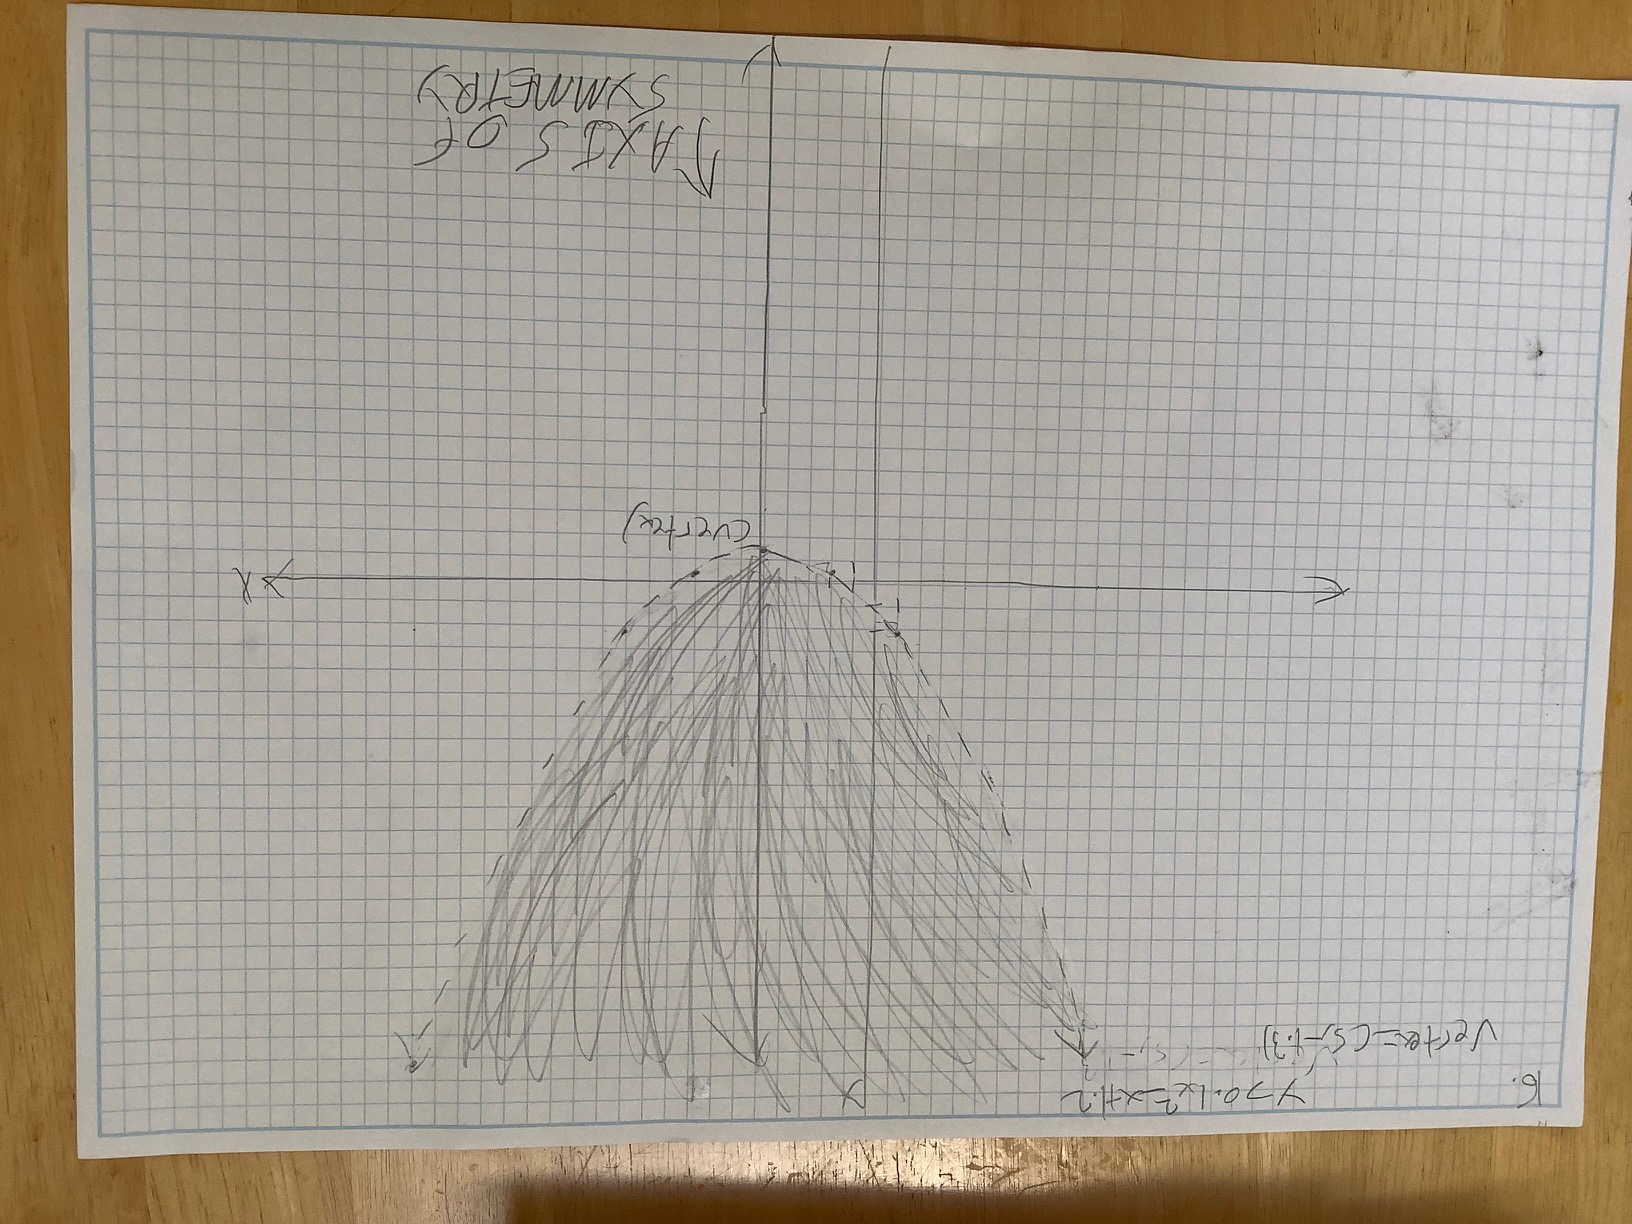
\includegraphics[width = 4in, height = 4in, angle = 180]{1.9picture1}

\section*{17}
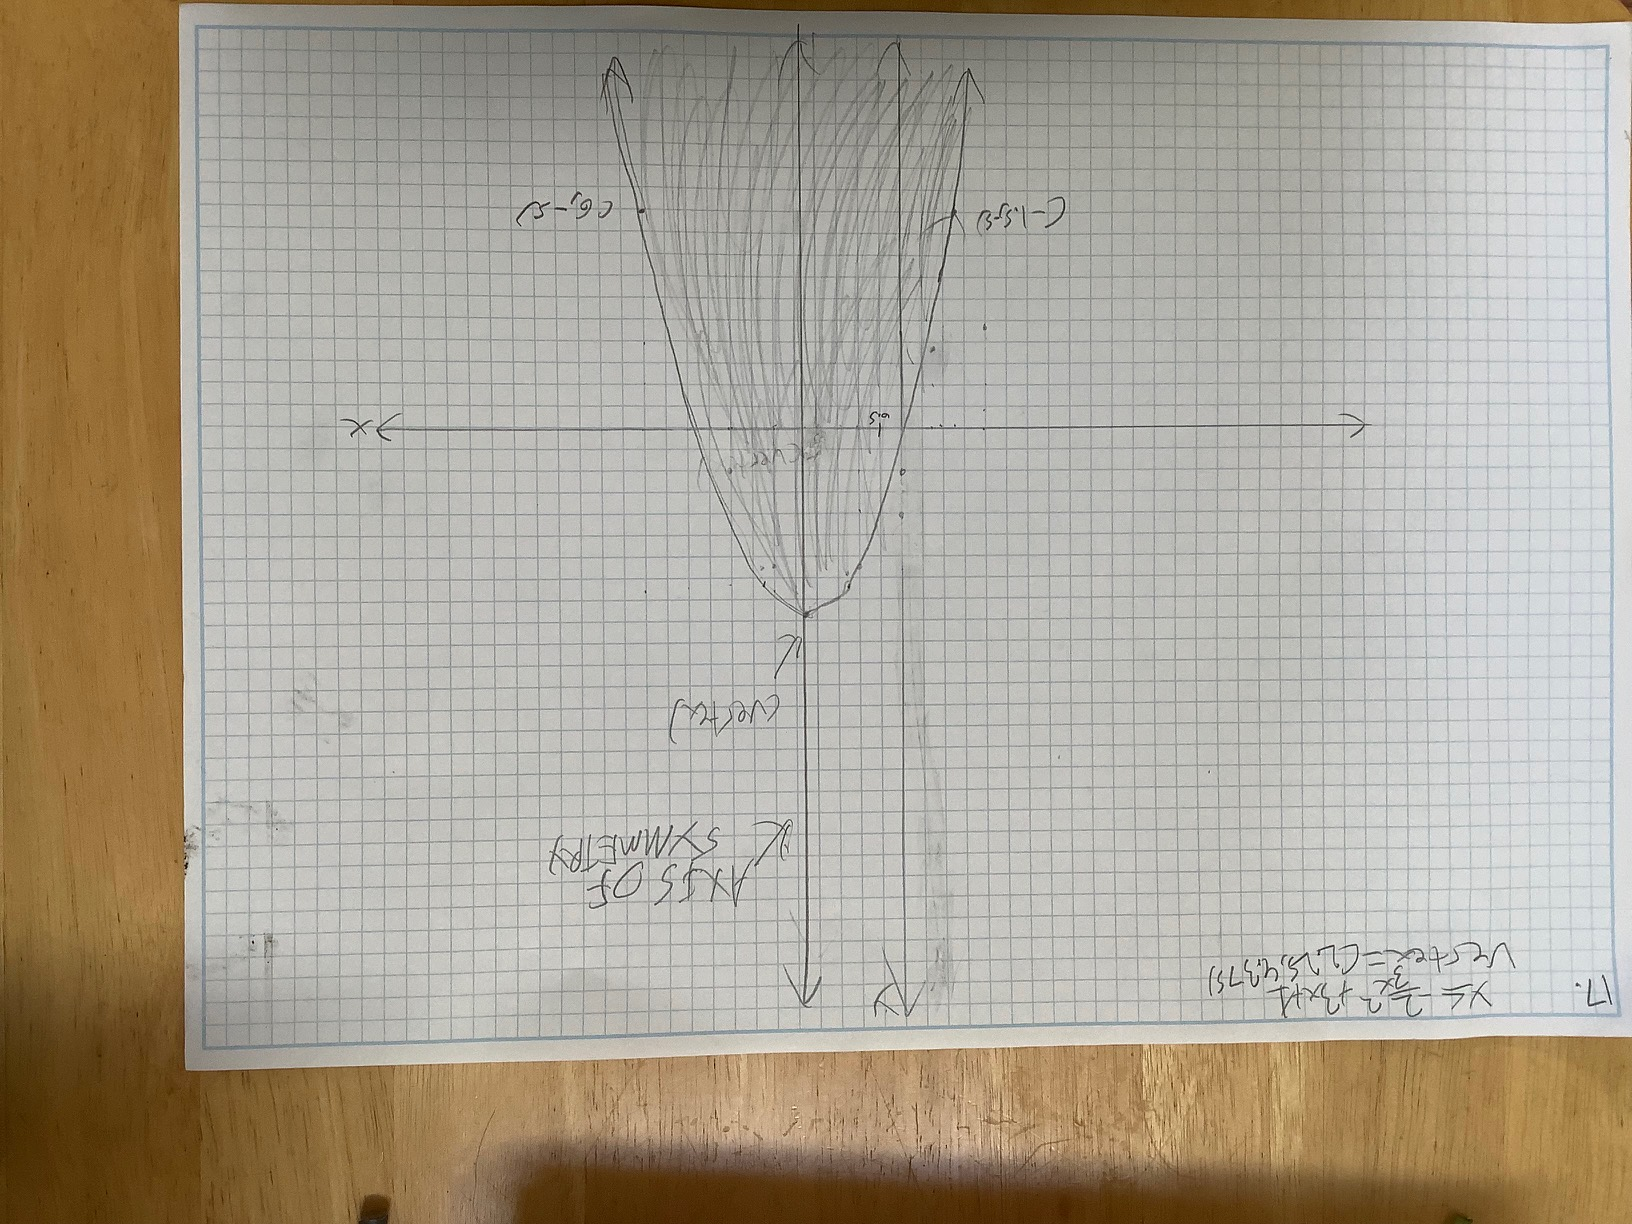
\includegraphics[width = 4in, height = 4in, angle = 180]{1.9picture2}

\section*{18}
The error here is that the graph has a dashed line. Because the equation has a $\le$, a solid line should be used. The answer would be correct if 
the shaded line was made to be solid.

\section*{19}
Here, the error is that the graph has all the values of $y$ less than the $y$ values for this quadratic equation shaded. This is incorrect, as 
the sign in this equation is a $\le$. This graph can be corrected by not shading the values below the parabola, but instead shading all of the values above 
the parabola.

\section*{24}
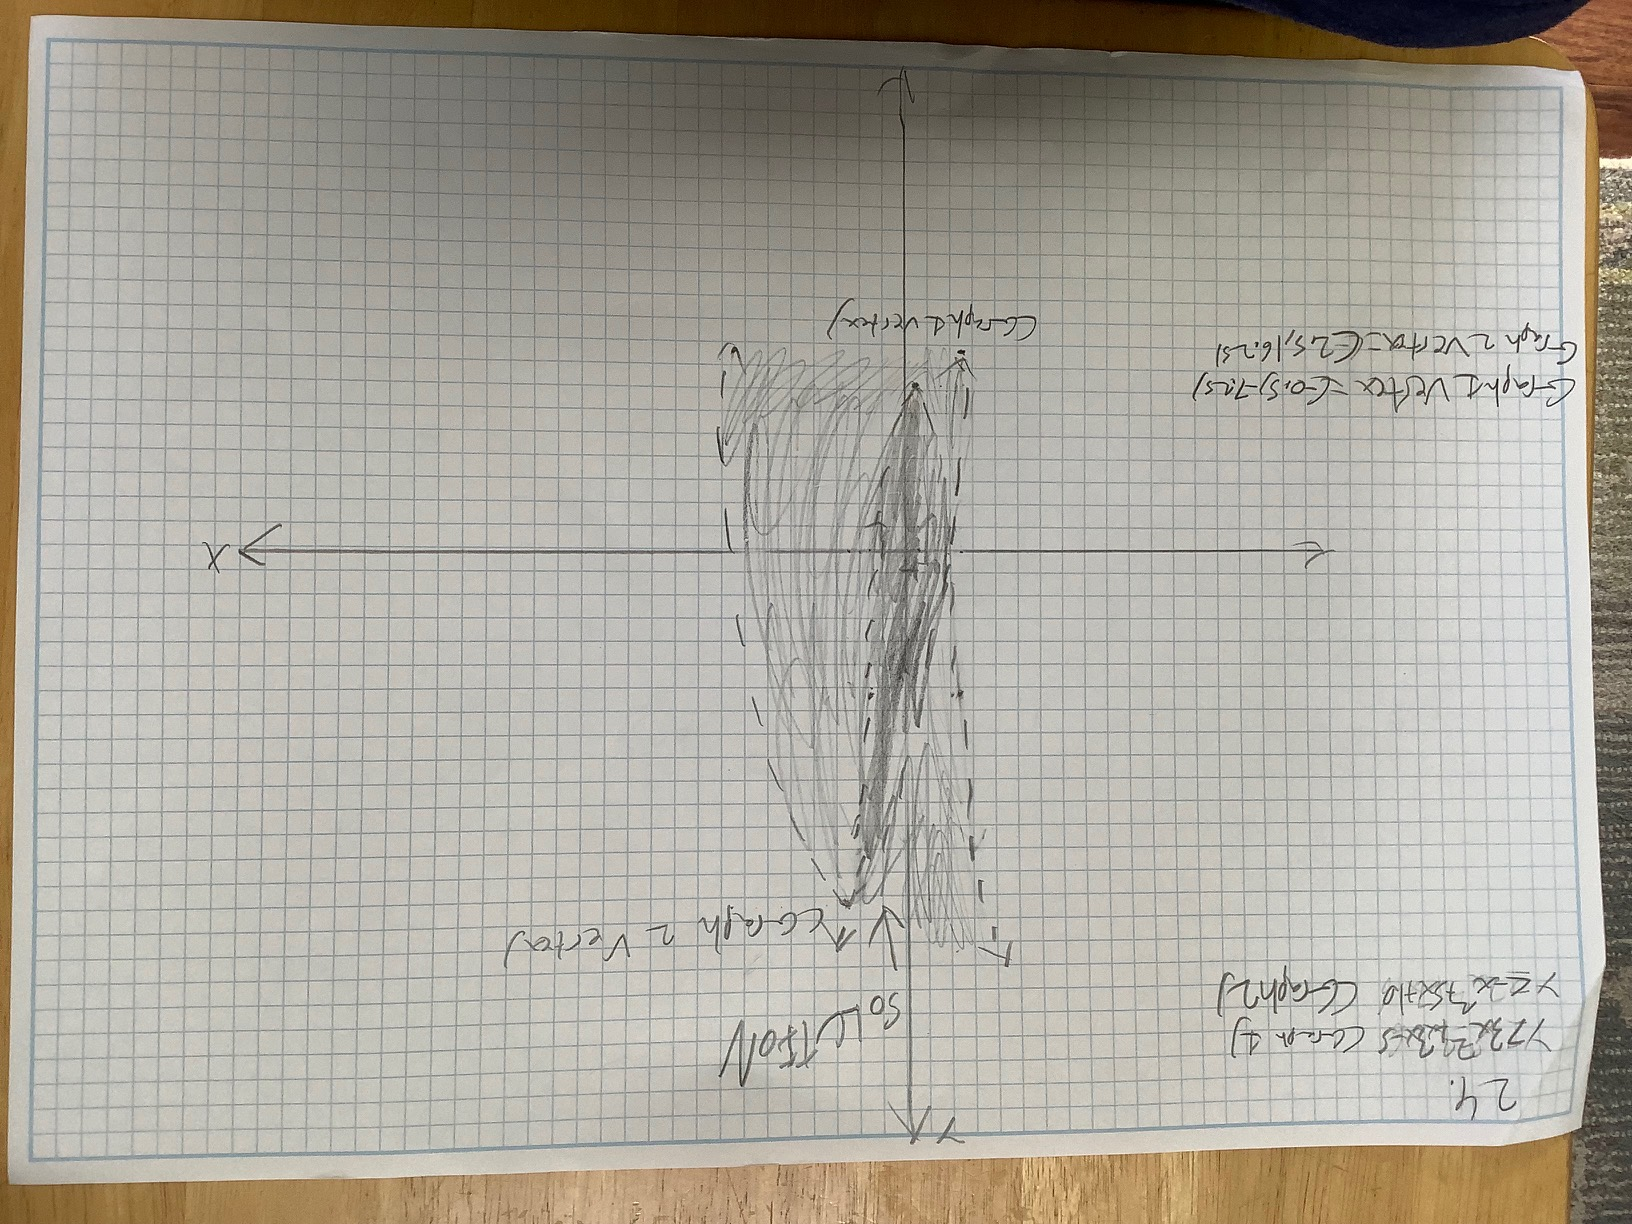
\includegraphics[width = 4in, height = 4in, angle = 180]{1.9picture3}

\section*{25}
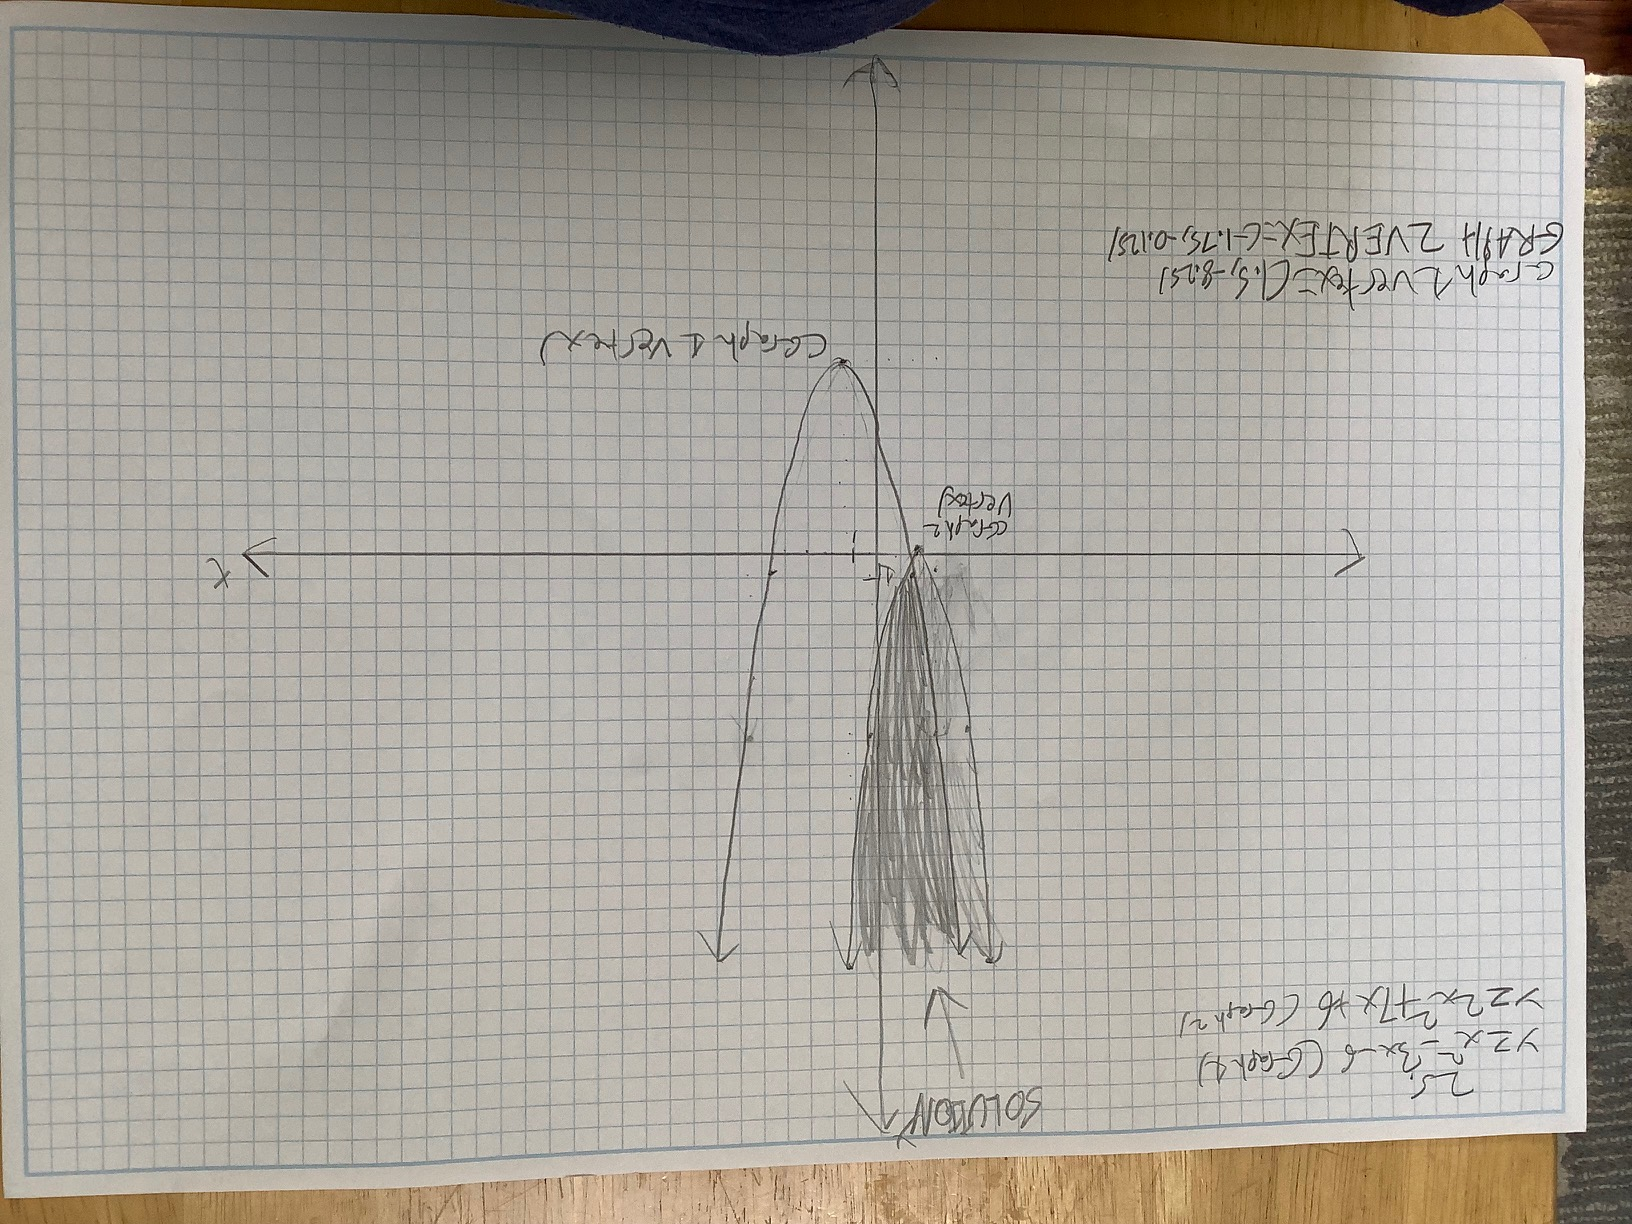
\includegraphics[width = 4in, height = 4in, angle = 180]{1.9picture4}

\section*{33}
Equation: $3x^2-6x-2\le 7\newline\rightarrow 3x^2-6x-9\le 0$
\begin{table}[h!]
        \begin{center}
                \begin{tabular}{l|c|c|c|c|c|c|c|r}
                        $x$ & $-2$ & $-1$ & $0$ & $1$ & $2$ & $3$ & $4$\\
                        \hline
                        $y$ & $15$ & $0$ & $-9$ & $-12$ & $-9$ & $0$ & $15$
                \end{tabular}
        \end{center}
\end{table}
From the table, we can see that the values of $y$ between $x=-1$ and $x=3$ inclusive are solutions of the inequality, 
thus meaning that the solution to the inequality 
is $-1\le x\le 3$

\section*{34}
Equation: $2x^2-6x-9\ge 11\newline\rightarrow 2x^2-6x-20\ge 0$
\begin{table}[h!]
        \begin{center}
                \begin{tabular}{l|c|c|c|c|c|c|c|c|c|c|r}
                        $x$ & $-3$ & $-2$ & $-1$ & $0$ & $1$ & $2$ & $3$ & $4$ & $5$ & $6$\\
                        \hline
                        $y$ & $16$ & $0$ & $-12$ & $-20$ & $-24$ & $-24$ & $-20$ & $-12$ & $0$ & $16$
                \end{tabular}
        \end{center}
\end{table}
From the table, we can see that the values of $y$ that are $\ge 0$ start from $\le -2$ as well as $\ge 5$. Thus, the solution of this inequality is 
that $x\le -2\vee x\ge 5$

\section*{42}
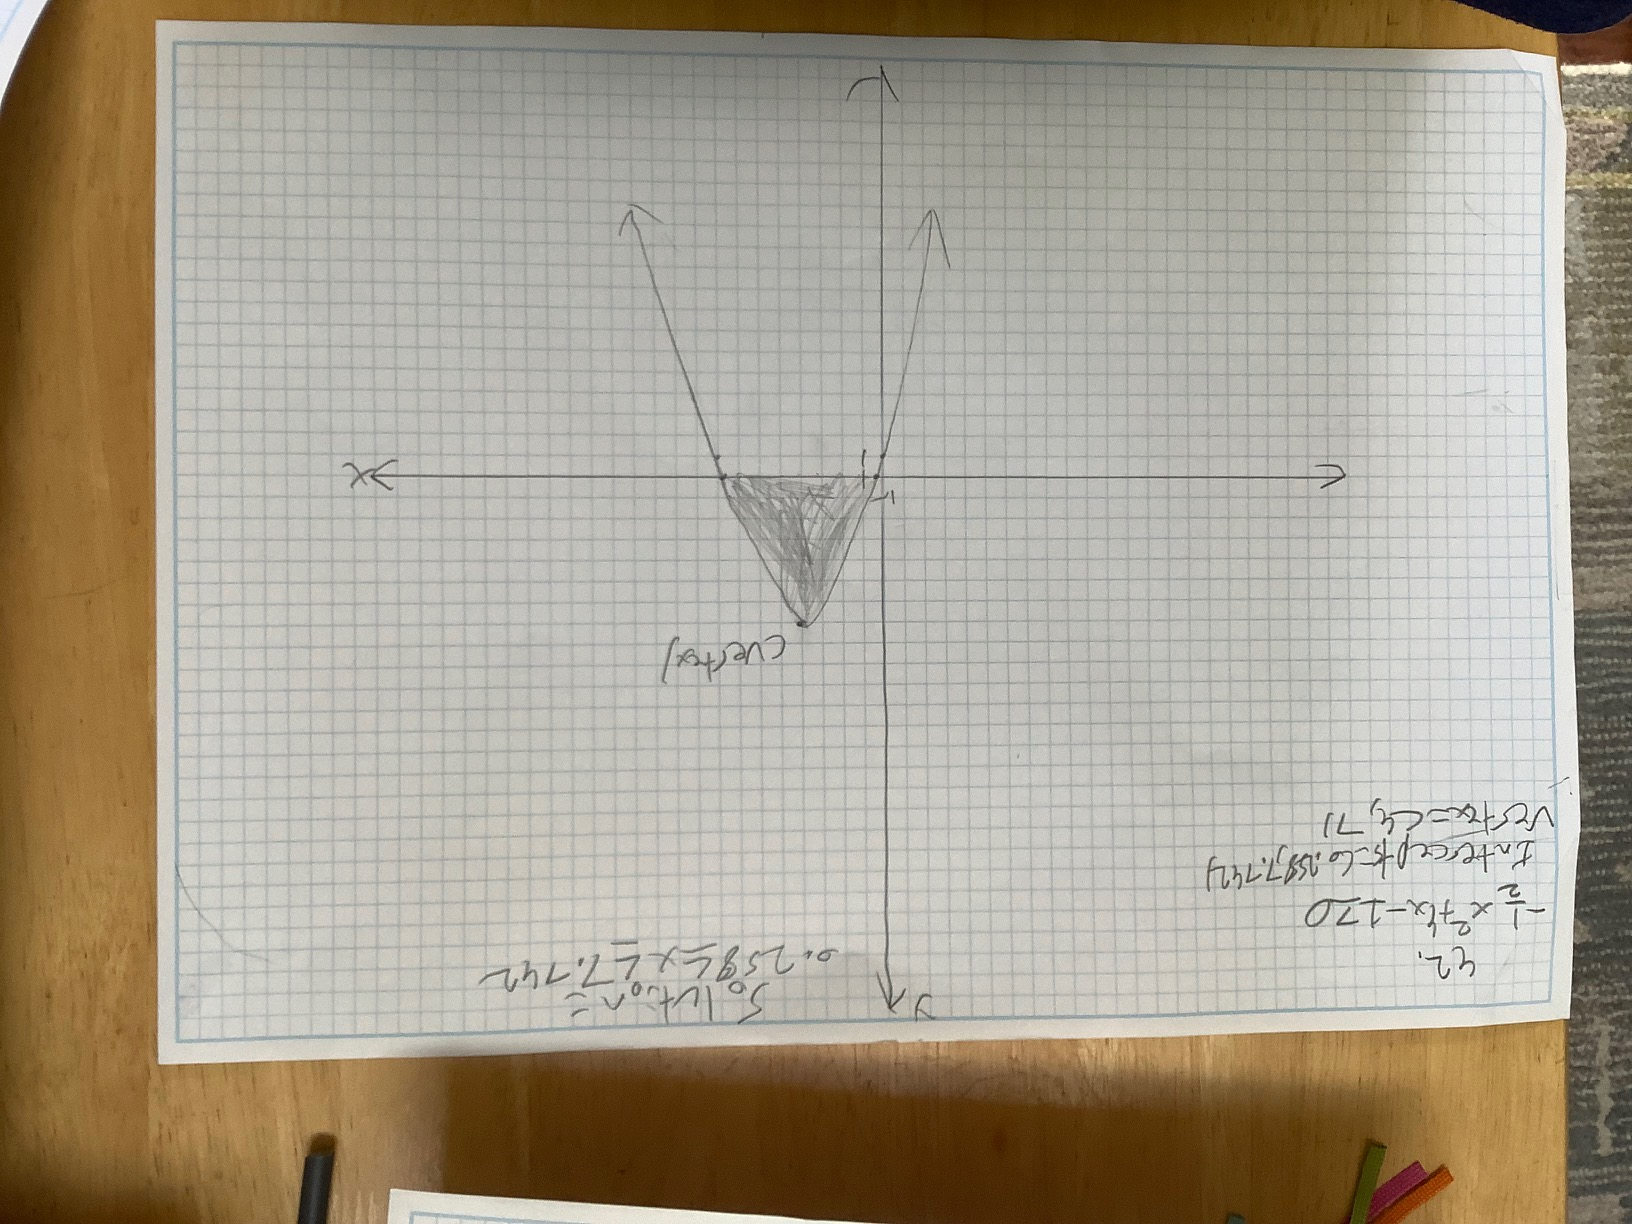
\includegraphics[width = 4in, height = 4in, angle = 180]{1.9picture5}

\section*{43}
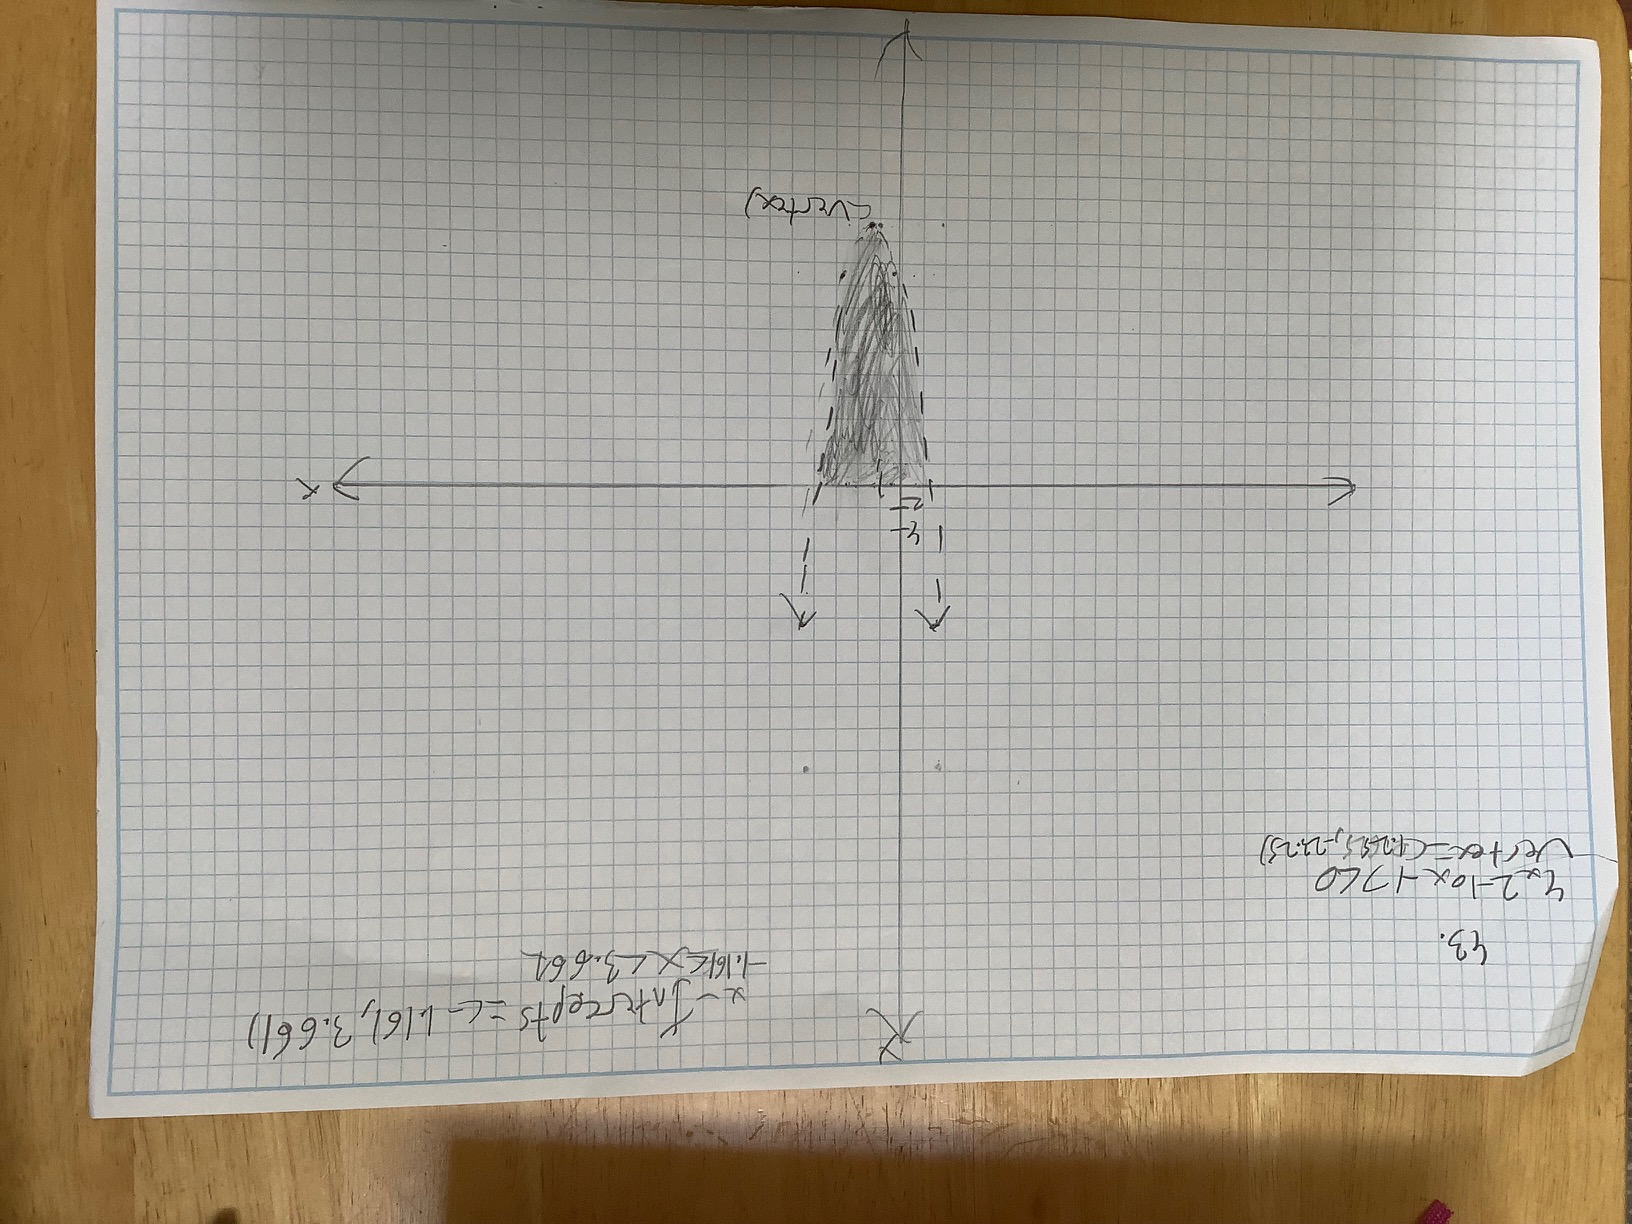
\includegraphics[width = 4in, height = 4in, angle = 180]{1.9picture6}

\section*{44}
$3x^2-x-4>0\newline\rightarrow 
(3x-4)(x+1)=0$ (Rewrite in standard form and factor) 
$\newline\rightarrow x=\frac{4}{3}\vee x=-1\newline$ because the graph opens up, $x<-1\vee x>\frac{4}{3}$, thus meaning tha the correct answer is A.

\section*{45}
$2x^2+9x\le 56\newline\rightarrow 
2x^2+9x-56\le 0\newline\rightarrow 
(2x-7)(x+8)=0$ (Rewrite in standard from and factor)
$\newline\rightarrow x=\frac{7}{2}\vee x=-8\newline$ because the graph opens up, and we are searching for those value $\le 0$, the solutions are 
$-8\le x\le \frac{7}{2}$ thus meaning the correct answer is B.

\section*{56}
$3x^2+1<15x\newline\rightarrow 
3x^2-15x+1<0\newline\rightarrow 
3x^2-15x+1=0$ (Rewrite in standard form)
$\newline\rightarrow x=\frac{15\pm\sqrt{(-15)^2-4(3)(1)}}{2(3)}\newline\rightarrow 
x=4.93\vee x=0.07$\newline Because the graph opens up, and we are searching for those values $<0$, the solutions are 
$0.07<x<4.93$

\section*{57}
$6x^2-5>8x\newline\rightarrow 
6x^2-8x-5>0\newline\rightarrow 
6x^2-8x-5=0$ (Rewrite in standard form)
$\newline\rightarrow x=\frac{8\pm\sqrt{(-8)^2-4(6)(-5)}}{2(6)}\newline\rightarrow 
x=1.797\vee x=-0.464$\newline Because the graph opens up, and we are searching for those values $>0$, the solutions are
$x<-0.464\vee x>1.797$

\section*{58}
(a): 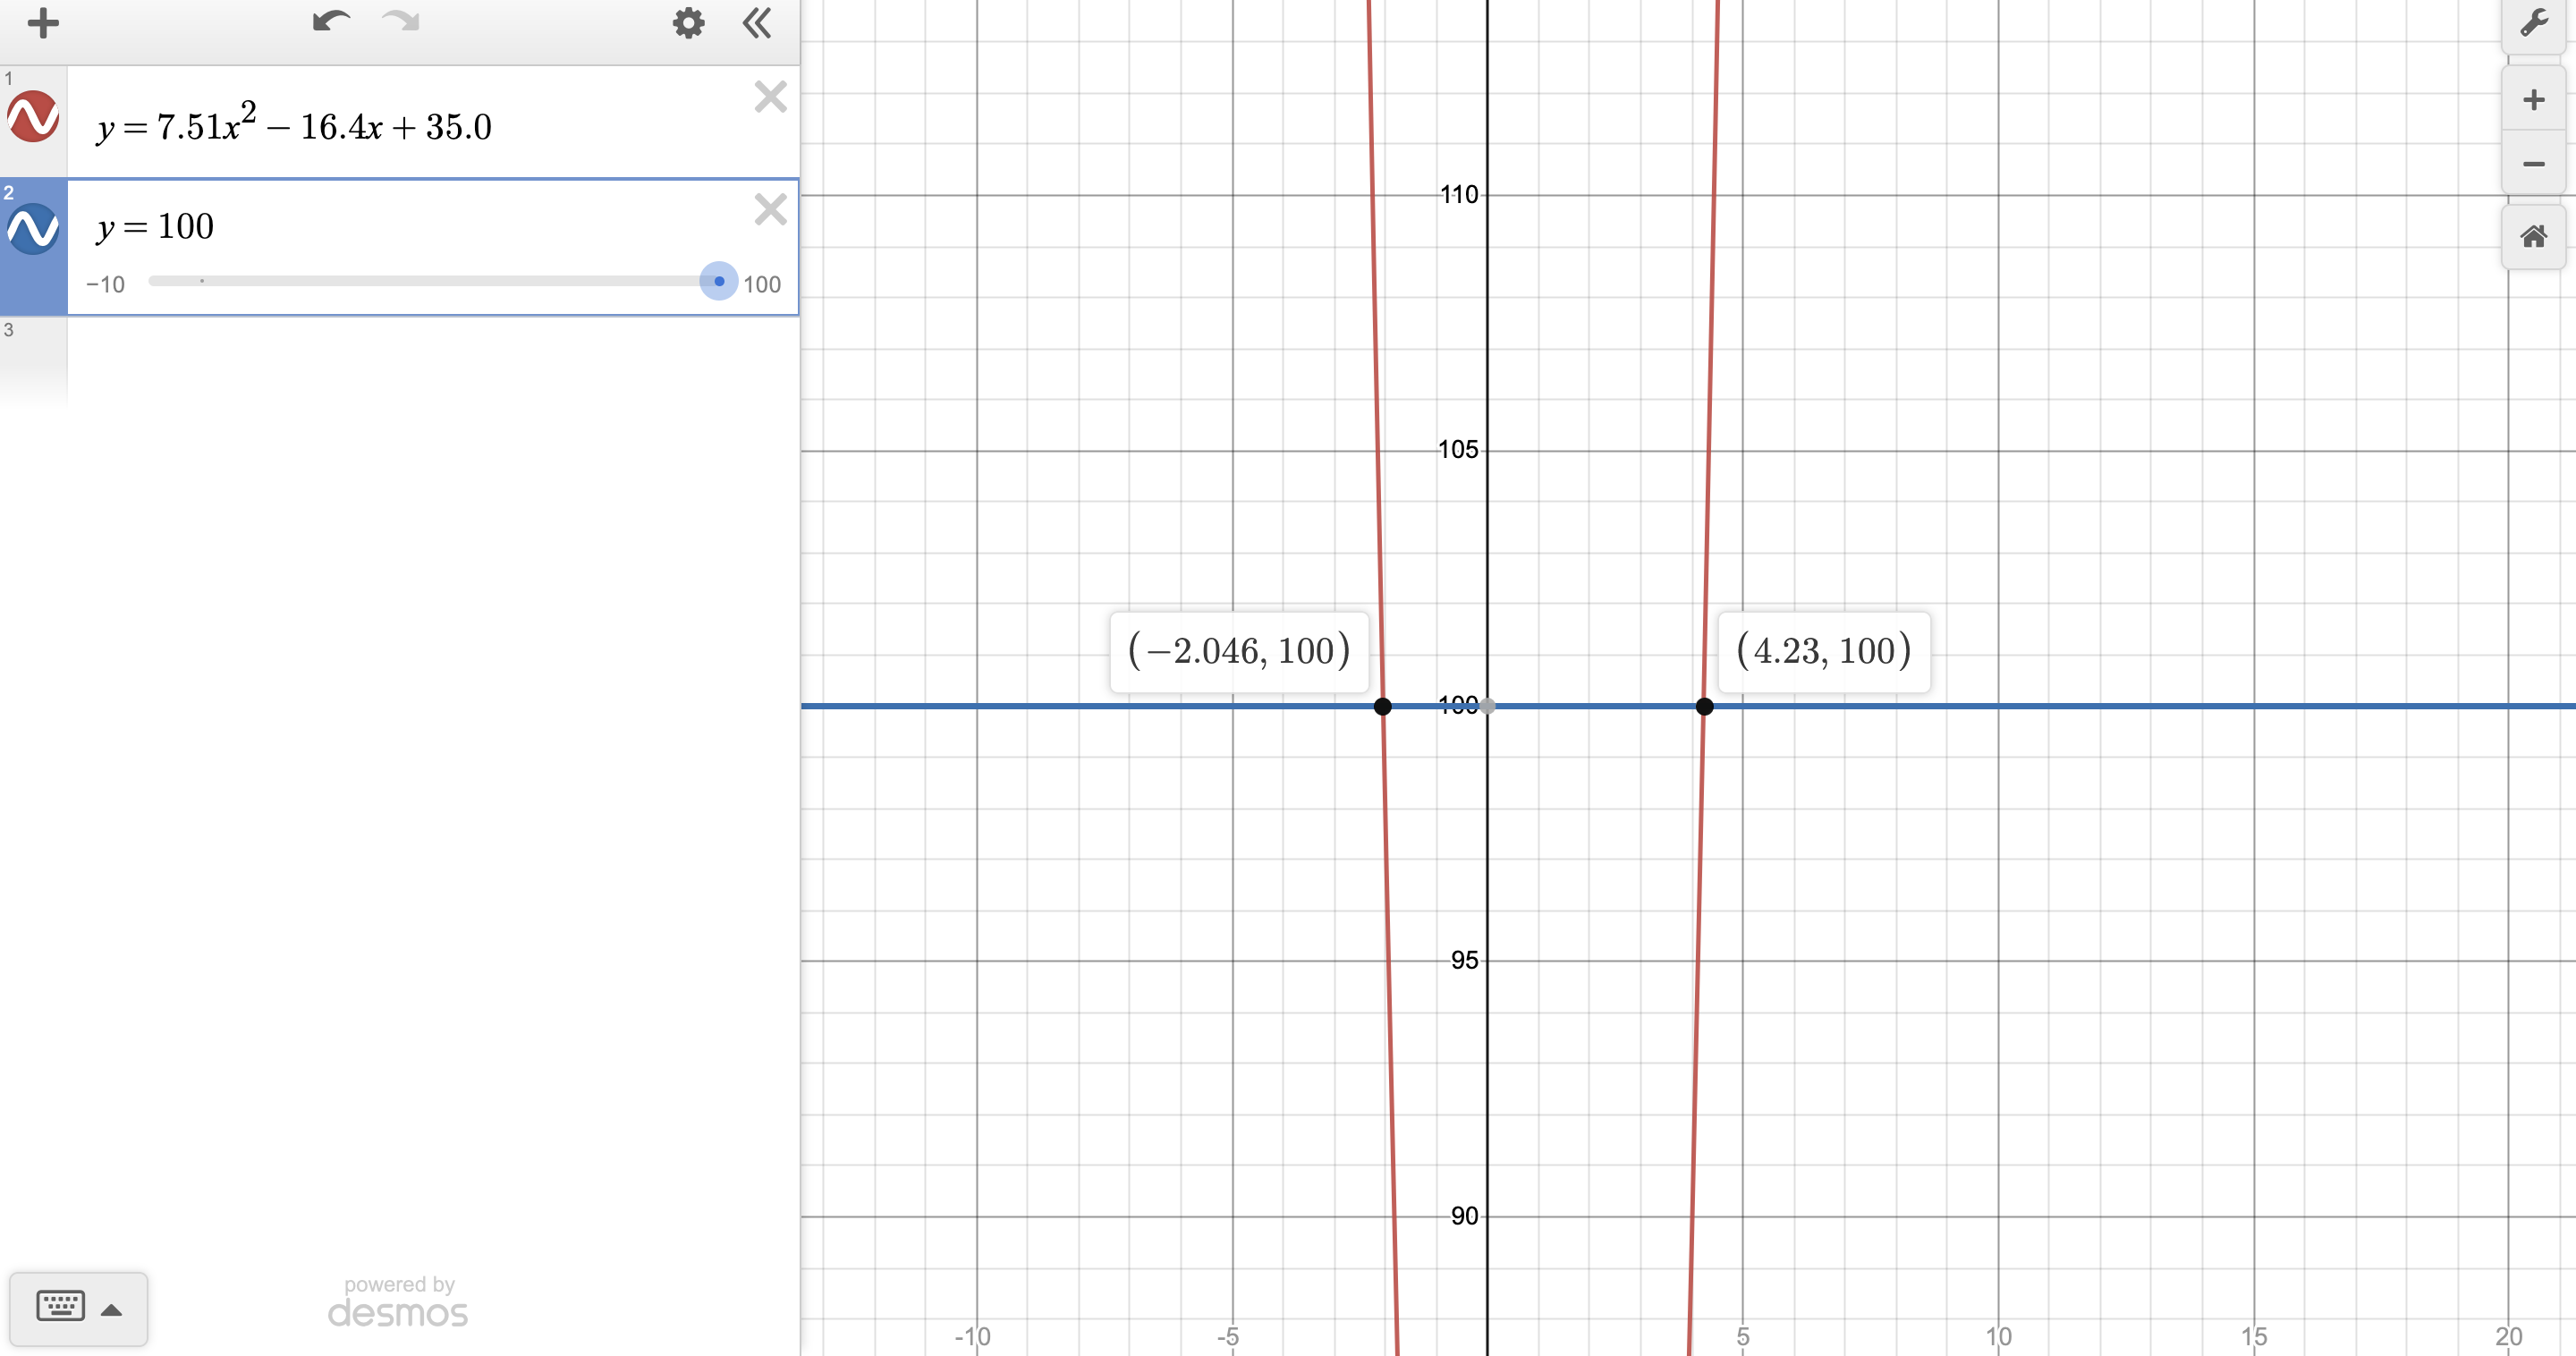
\includegraphics[width = 4in, height = 4in]{1.9picture7}
\newline (b): 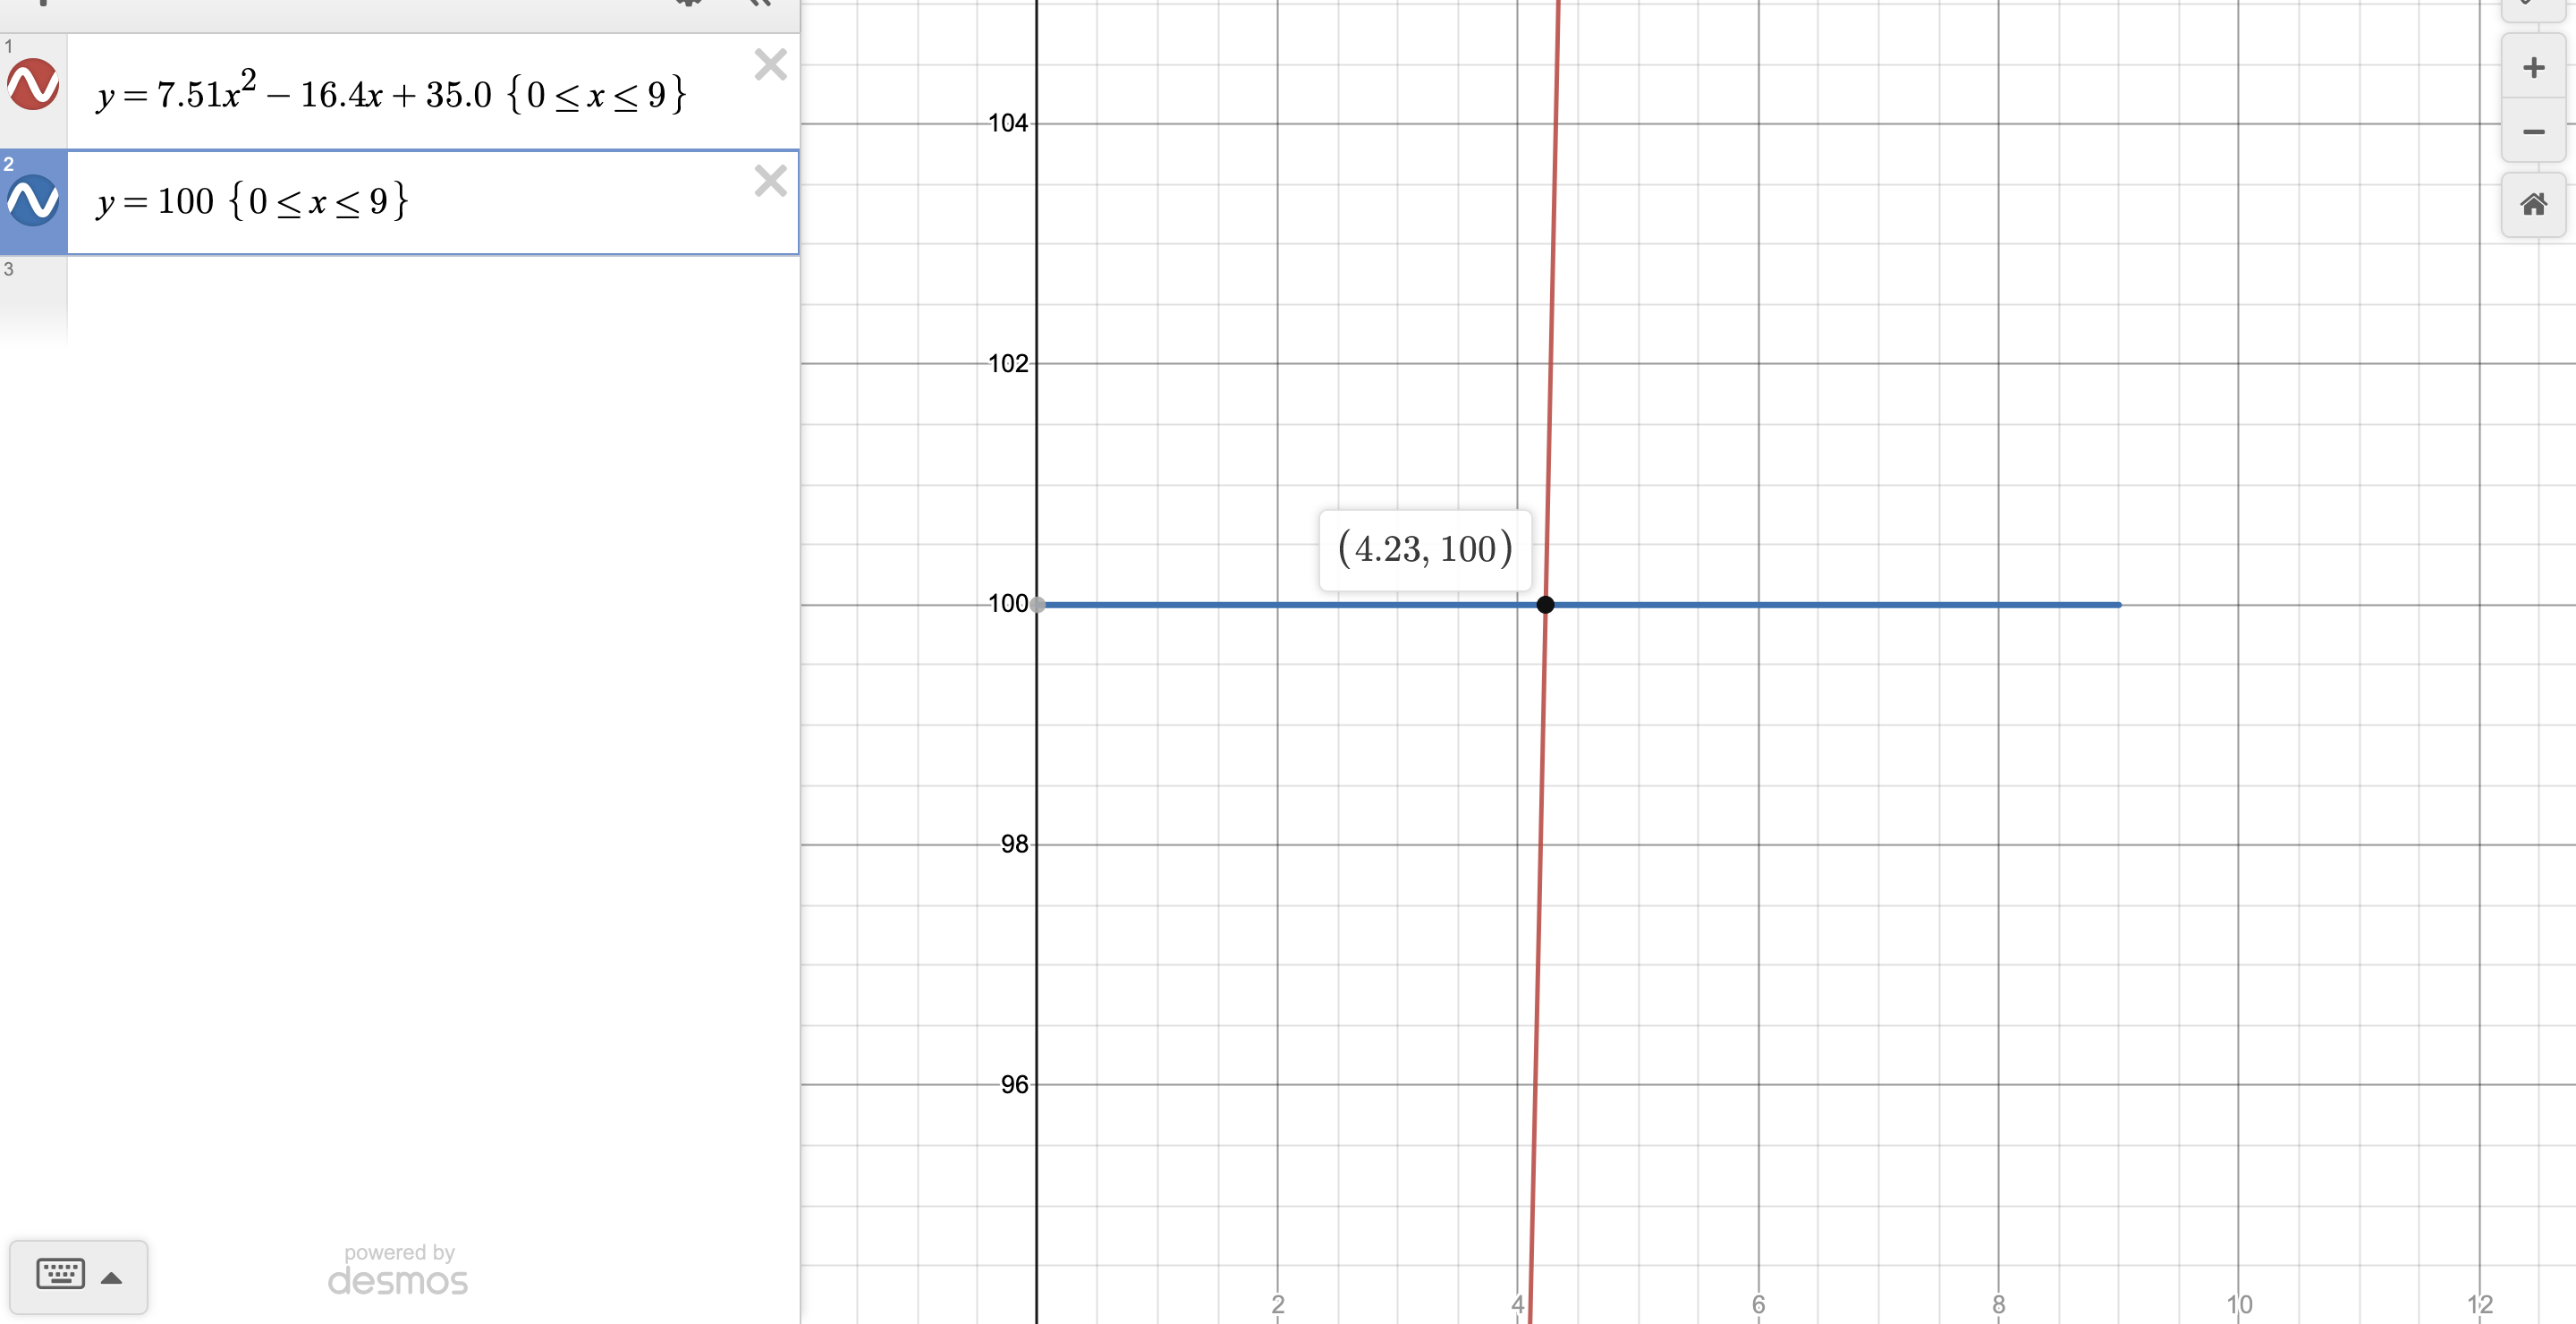
\includegraphics[width = 4in, height = 4in]{1.9picture8}
\newline (c): From the graph in part $b$, one can see that the intersection of these two functions is $(4.23,100)$.\newline
(d): The red graph represents the number o participating teams. Well, we can see that the values that satisfy this start at $x>4.23$ Well, we also know 
the fact (see the example) that $0\le x\le 9$, thus meaning the actual solutions to the inequality are $4.23<x\le 9$. Hence, because we are starting in the 
year 1992, the solutions are between the years $4.23$ and $9$ years after $1992$, that is, from $1996-2001$.

\section*{66}
$5x^2+x-7<3x^2-4x\newline\rightarrow 
2x^2+5x-7<0\newline\rightarrow 
2x^2+5x-7=0$ (Rewrite in standard form)
$\newline\rightarrow (2x+7)(x-1)=0\newline\rightarrow 
x=-\frac{7}{2}\vee x=1$\newline Because the graph of this function opens upwards, and we are finding those values such that $x<0$, 
$-\frac{7}{2}<x<1$

\section*{67}
$6x^2-5x+2<-3x^2+x\newline\rightarrow 
9x^2-6x+2<0\newline\rightarrow 
9x^2-6x+2=0$ (Rewrite in standard form, in order to find the intercepts)
$\newline\rightarrow x=\frac{6\pm\sqrt{(-6)^2-4(9)(2)}}{2(9)}\newline\rightarrow 
x=\frac{6\pm\sqrt{-36}}{18}\newline\rightarrow 
x=\frac{6\pm 6i}{18}\newline\rightarrow 
x=\frac{1}{3}+\frac{1}{3}i\vee x=\frac{1}{3}-\frac{1}{3}i$\newline Because the graph of this function opens upwards, and we are finding those values such 
that $x<0$, $\frac{1}{3}-\frac{1}{3}i<x<\frac{1}{3}+\frac{1}{3}i$

\section*{68}
An inequality with these solutions could originate from an inequality have an equation that, when put into standard form, has the intercepts $-2$ and 
$5$. One such equation is $(x+2)(x-5)\newline\rightarrow x^2-3x-10$. Because the given answers to the inequality are $x<-2\vee x=5$, an inequality 
with the given solutions could be $x^2-3x-10>0\vee x^2-3x>10$

\section*{69}
(a): 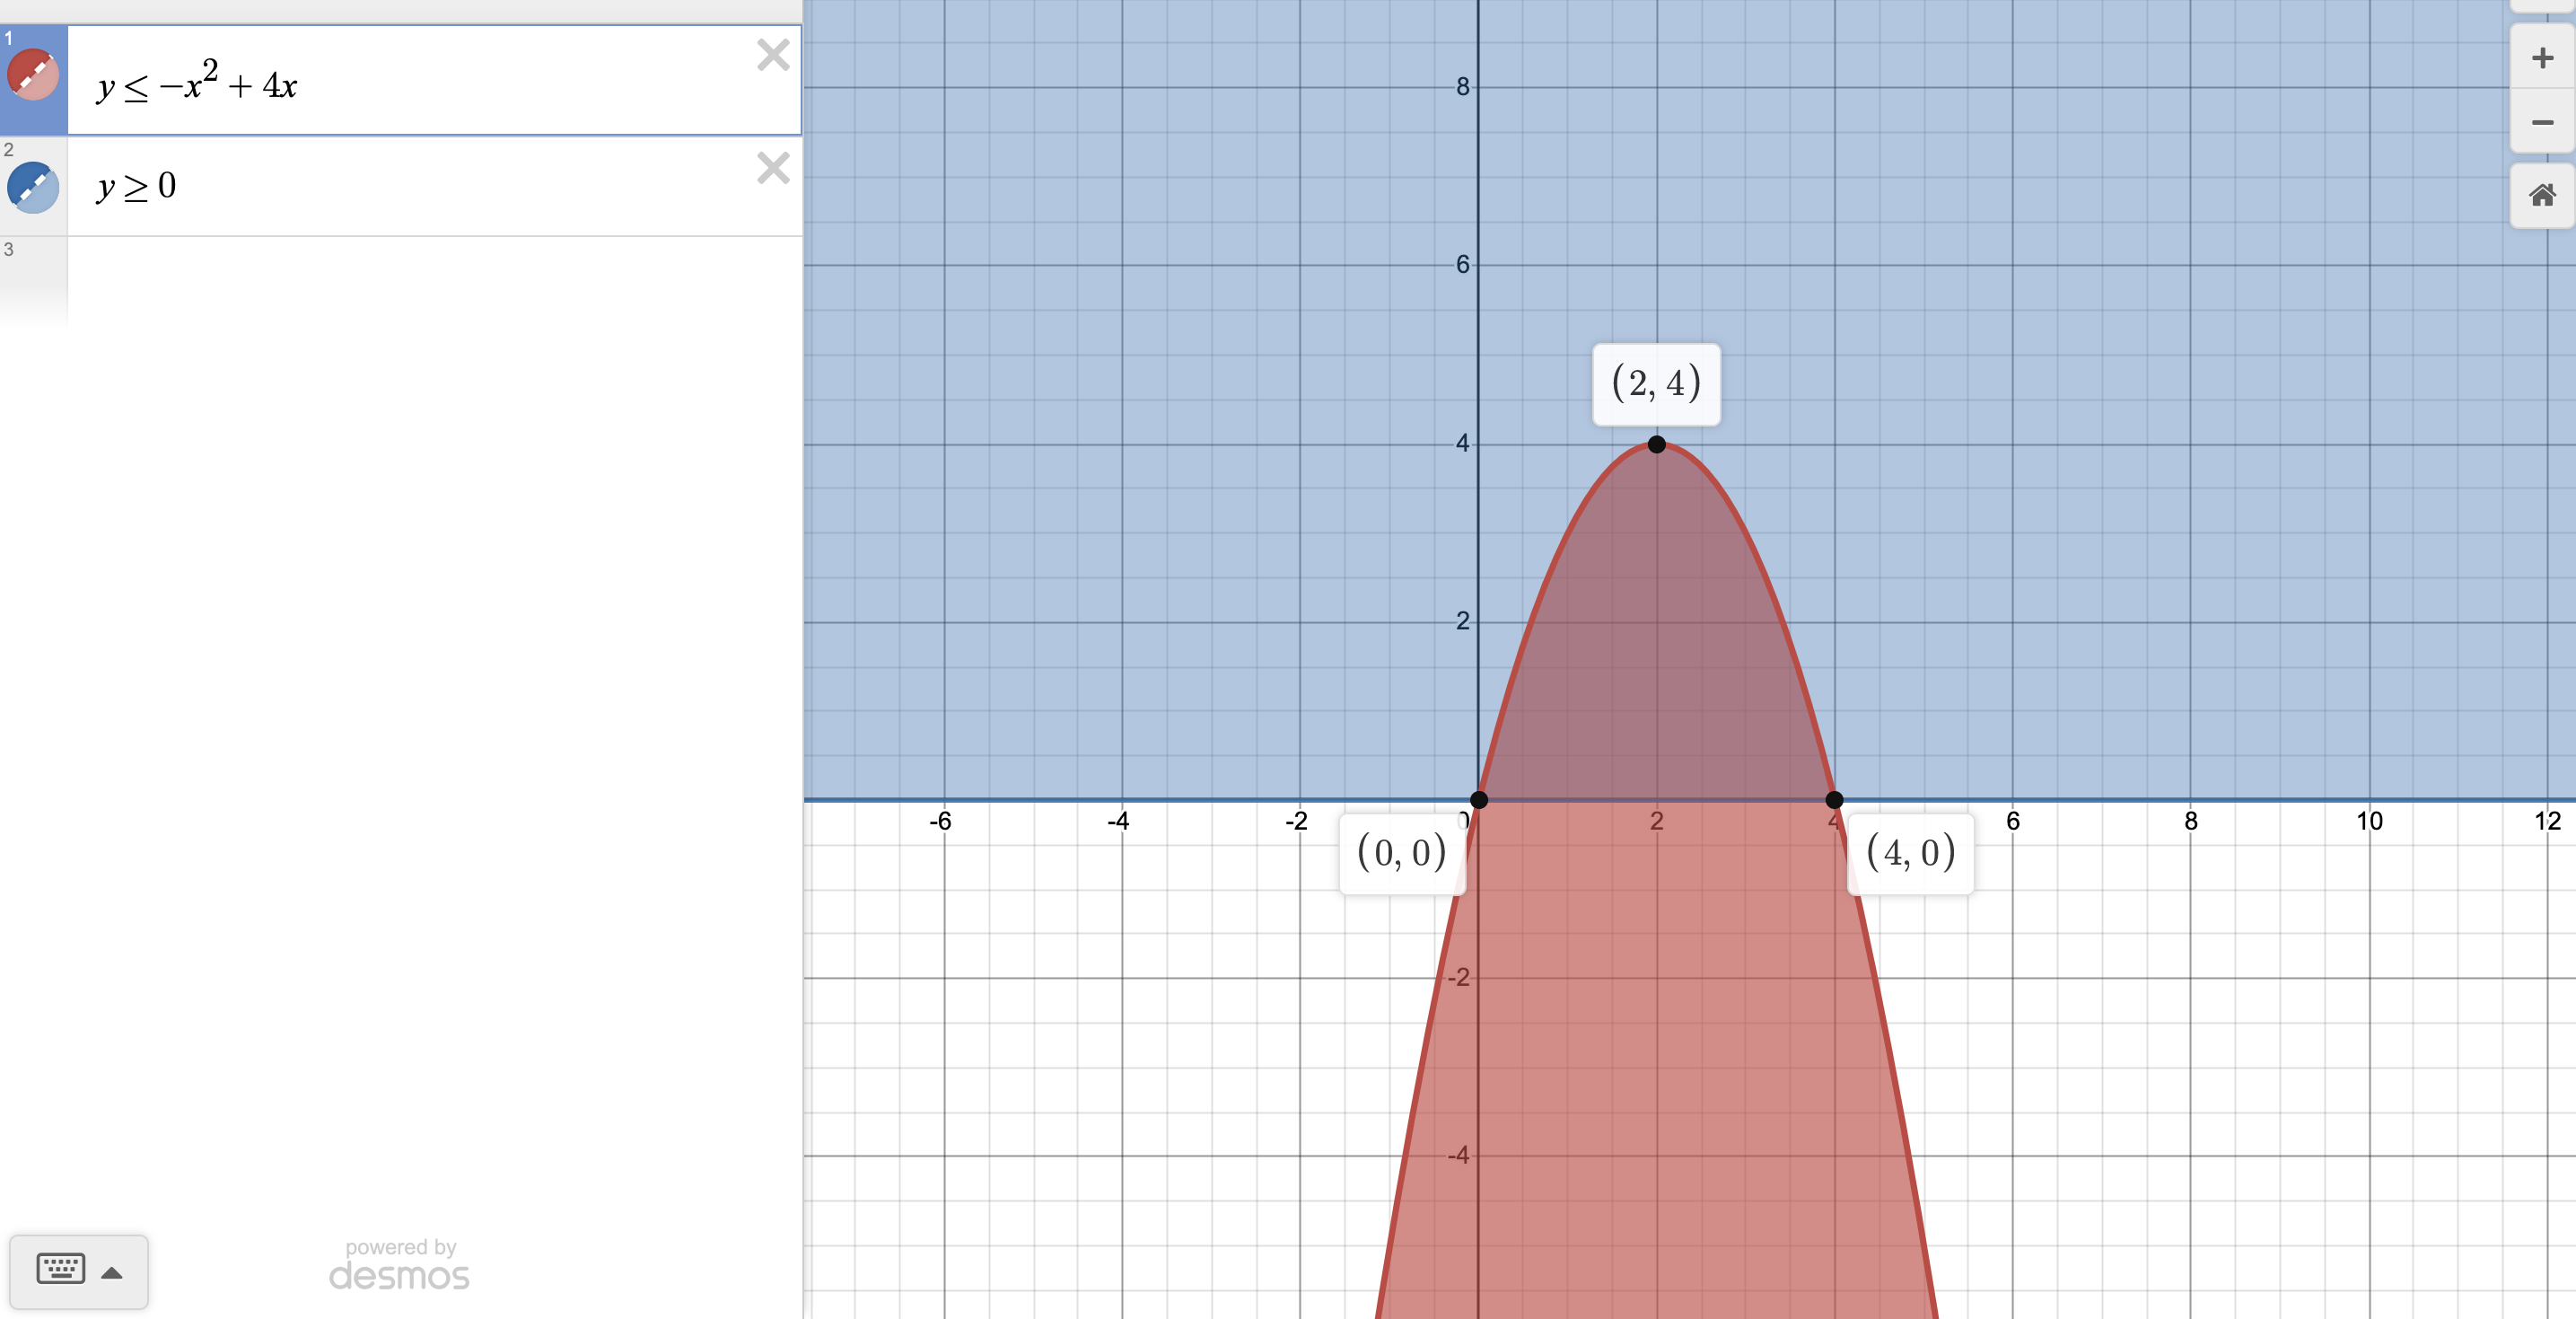
\includegraphics[width = 4in, height = 4in]{1.9picture10}\newline From the graph, we can see that $h=4-0=4$, while $b=4-0=4$, thus meaning 
$A=\frac{2}{3}\times 4\times 4=\frac{32}{3}$\newline
(b): 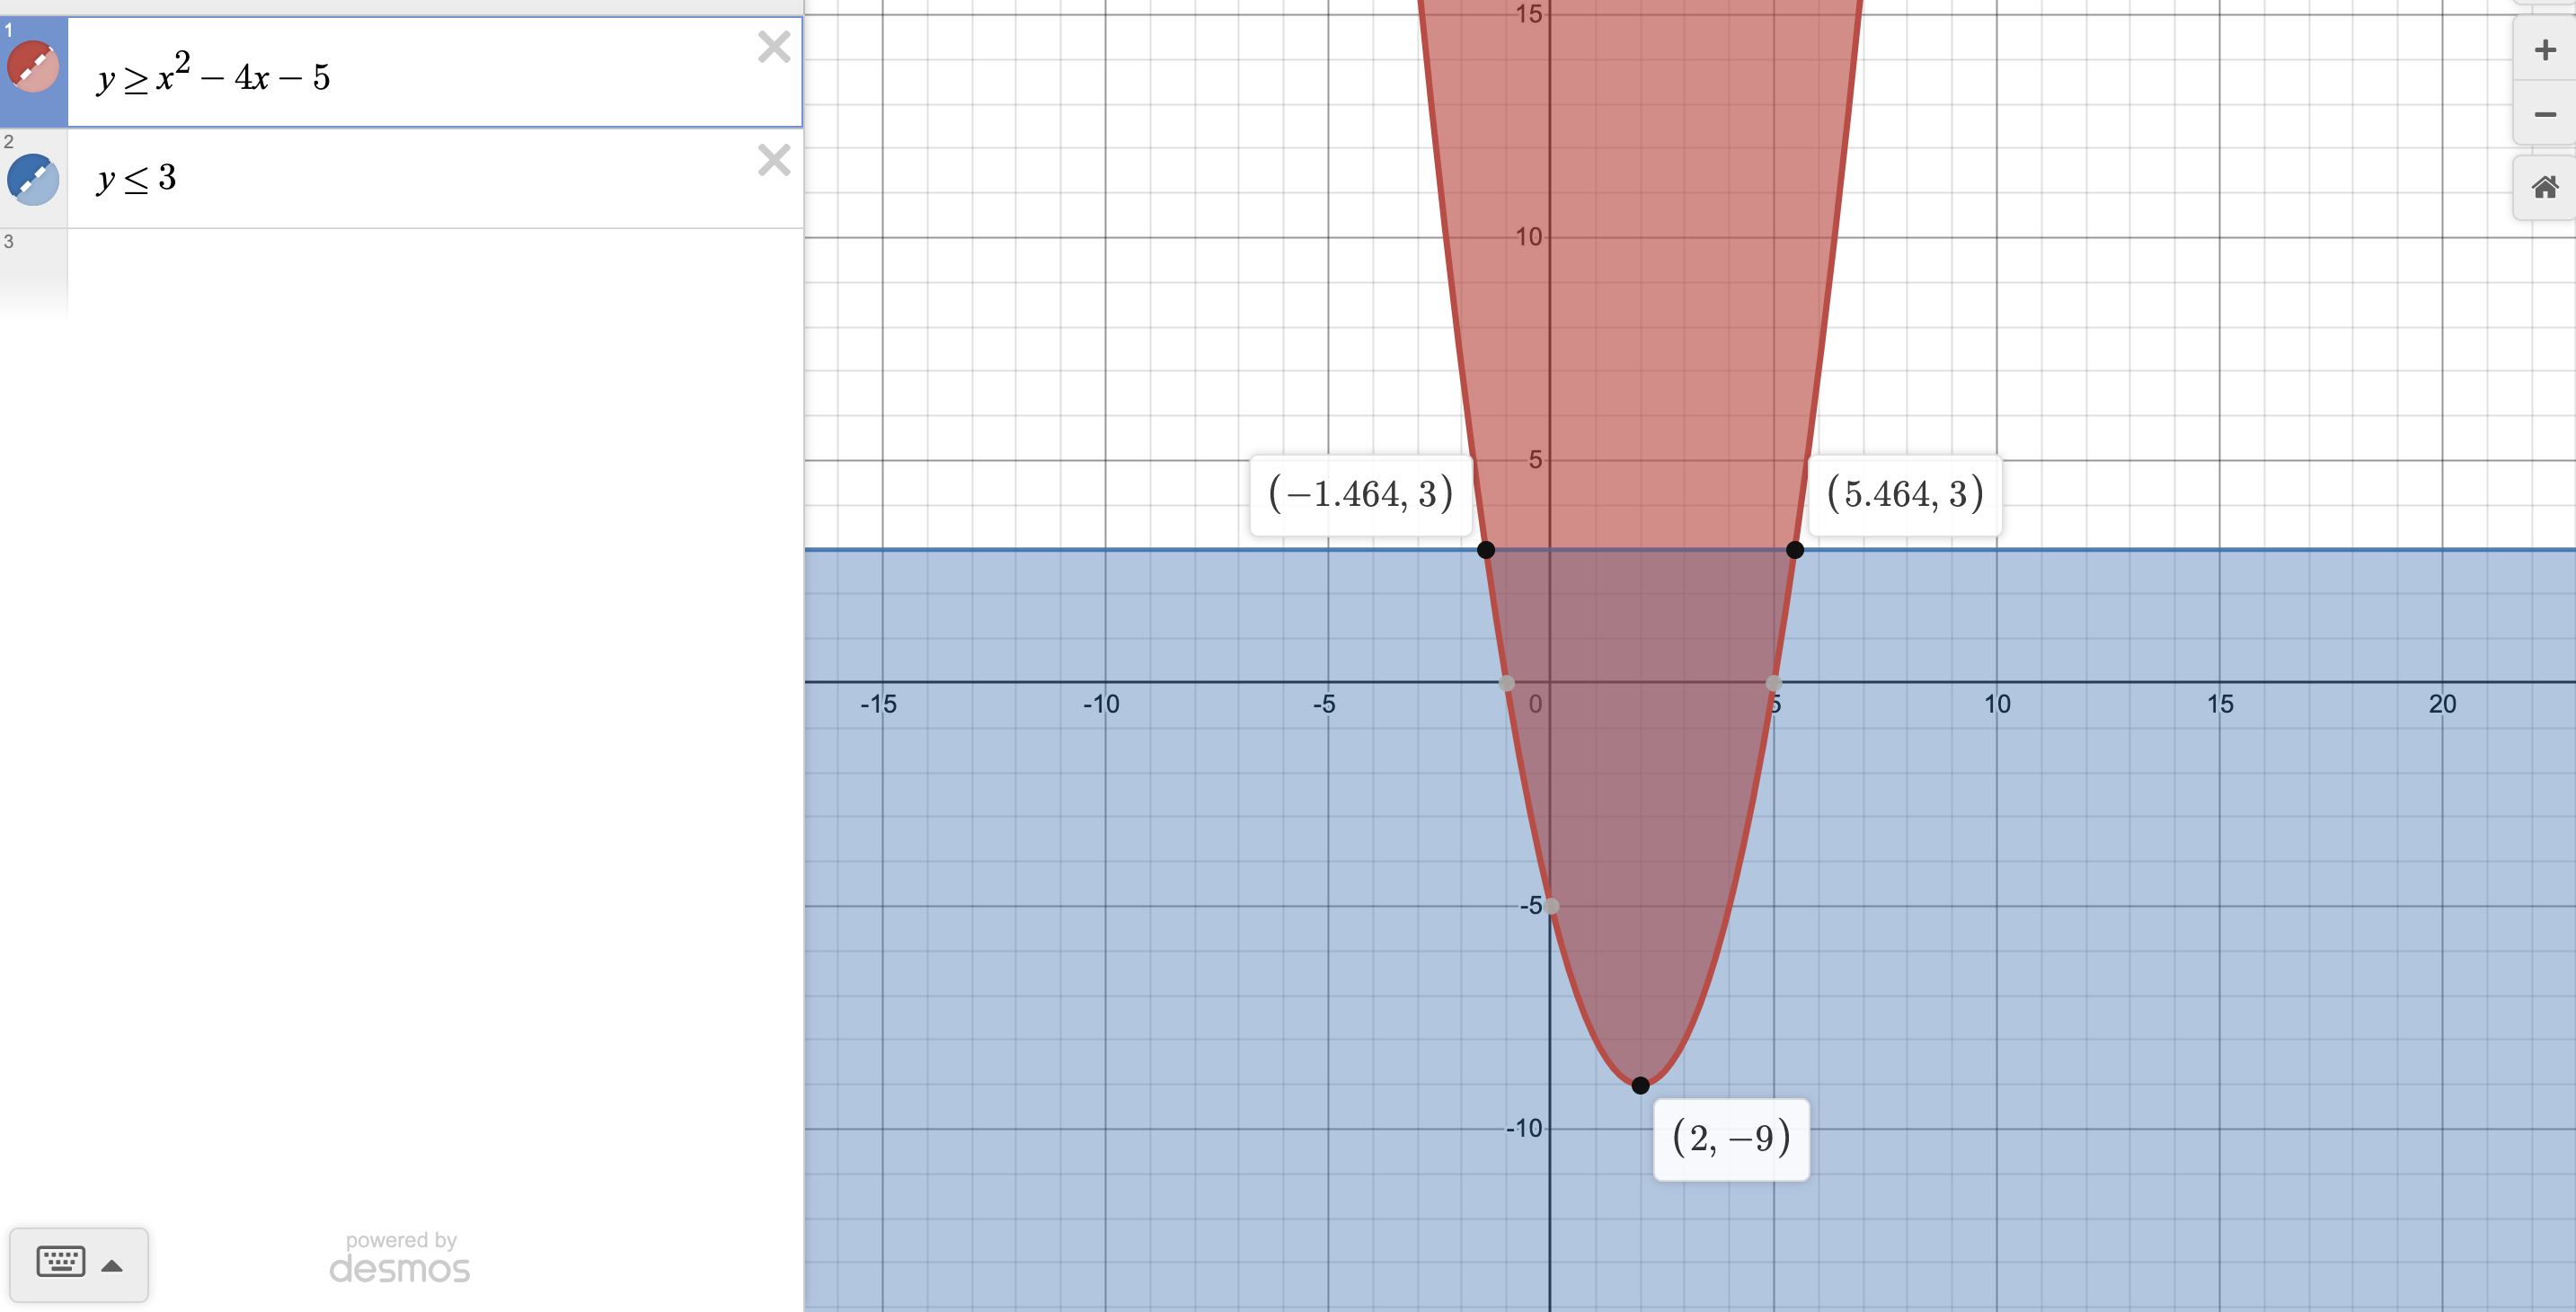
\includegraphics[width = 4in, height = 4in]{1.9picture11}\newline From the above graph, we can see that $h=|-9-3|=12$, while $b=5.464+1.464=6.928$, 
thus meaning $A=\frac{2}{3}(6.928)(12)=55.424$ 


\section*{72}
We are given that the road is $52$ meters high. Thus, an equation that satisfies this situation is $-0.00211x^2+1.06x\ge 52$\newline We can solve this 
algebraically, by finding the two solutions of the equation $-0.00211x^2+1.06x-52=0$:\newline 
$x=\frac{-1.06\pm\sqrt{1.06^2-4(-0.00211)(-52)}}{2(-0.00211)}\newline\rightarrow 
x=55.01\vee x=-1.887\newline\rightarrow$ 
Then, we check a value greater than $55.01$ to check if it satisfies the equation: $-0.00211(56.01)^2+1.06(56.01)\ge 52\newline\rightarrow 
-6.64+59.37\ge 52\newline\rightarrow 
52.73\ge 52$\newline 
and thus, we can conclude that $x\ge 55.01$ However, we cannot similarly conclude that $x\le -1.887$ This is because $x$ measures the distance 
in meters from the left pylon, which cannot be a negative value. Hence, the final answer is that the arch is above the road for the values 
$x\ge 55.01$

\section*{73}
The two equations that can represent this situtation are $0.00170x^2+0.145x+2.35\ge 10$ and $0\le x\le 40$\newline with this in mind, we can solve 
the equation $0.00170x^2+0.145x-7.65=y\newline\rightarrow 
x=\frac{-0.145\pm\sqrt{0.145^2-4(0.00170)(-7.65)}}{2(0.00170)}\newline\rightarrow 
x=36.84\vee x=-122.13$\newline 
because only positive values make sense here, the solution $x\le -122.13$ is ruled, meaning the solution is $x\ge 36.84$. Then, we need to adjust this 
solution to work for the given domain of $0\le x\le 40$. Well, $x\ge 40$ means $0\le x$, so the only change to the solution that has to be made 
is to add the additional requirenment that $x\le 40$. Hence, the final solution is that $36.84\le x\le 40$ 

\section*{74}
(a): Because the domain of both equations are the same, the domain of the equation $A(x)<V(x)$ is also $16\le x\le 70$ The inequality that models 
this situation is:\newline 
$0.0051x^2-0.319x+15<0.005x^2-0.23x+22\newline\rightarrow 
0.0001x^2-0.089x-7<0,\ 16\le x\le 70\newline$
(b): I could not understand the point of creating such a table, because the intercepts of the equation listed above are not even in between any of the 
values of $x$ from $16$ to $70$.\newline
(c): 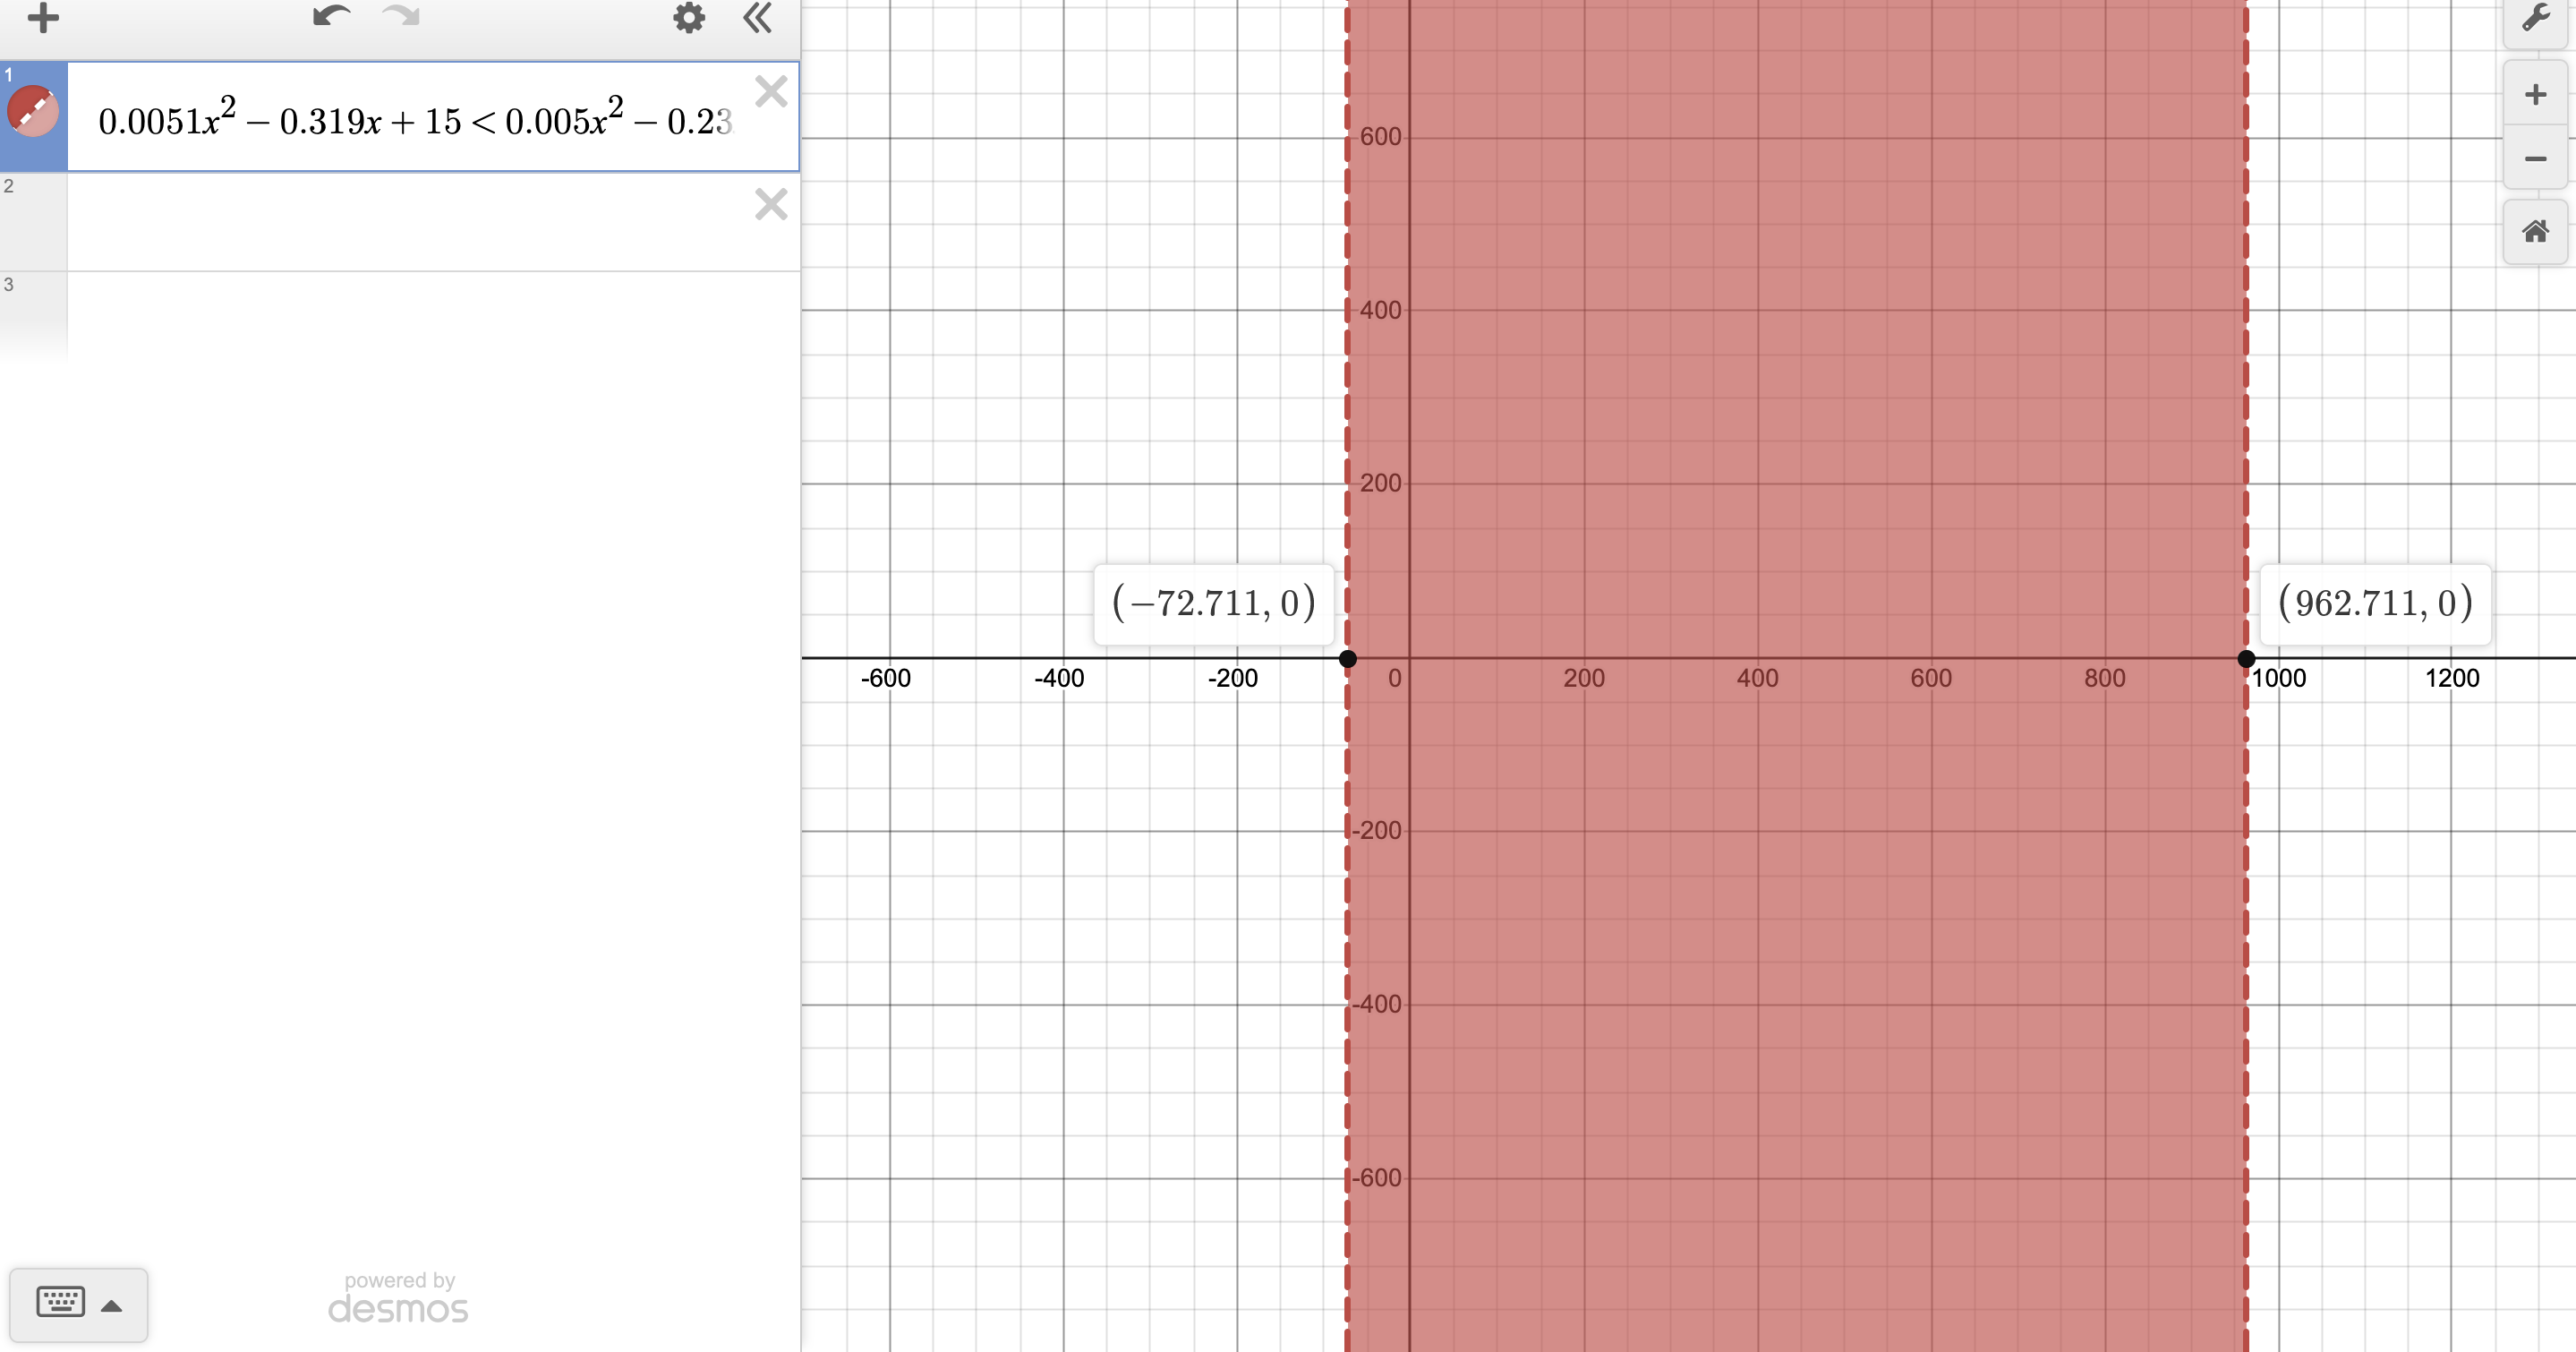
\includegraphics[width = 4in, height = 4in]{1.9picture9}\newline Based on the given domain of $16\le x\le 70$, it can be seen that 
all values from $16$ to $70$ are included in the solution, thus meaning that the solution to the equation should be $16\le x\le 70$.\newline
(d): Because the result from $c$ says that $A(x)<V(x)$ for all the values in the given domain of $16\le x\le 70$, it can be assumed that a driver would 
react slower to the siren than to the traffic light.


\section*{75}
(a): To solve this part of the problem, we need to solve the inequality $-0.0540x^2+1.43x<8\newline\rightarrow 
-0.0540x^2+1.43x-9<0$\newline To solve this inequality, we consider the equation $-0.0540x^2+1.43x-8=0$ and we find its intercepts:\newline 
$x=\frac{-1.43\pm\sqrt{1.43^2-4(-0.0540)(-8)}}{2(-0.0540)}\newline\rightarrow 
x=8.03\vee x=18.45$\newline So, the solution to this inequality is that $x\le 8.03\vee x\ge 18.45$\newline Now, because kicking the ball a negative value 
does not make sense, the solution should be changed to $0\le x\le 8.03\vee x\ge 18.45$\newline Also, it does not make sense to have the ball kicked 
to equal a negative $y$ value, so we need to find the intercepts of the equation $-0.0540x^2+1.43x-8<0\newline\rightarrow 
x=\frac{-1.43\pm\sqrt{1.43^2-4(-0.0540)(-8)}}{2(-0.0540)}\newline\rightarrow 
x=0\vee x=26.48$ Because this graph points downwards, all the values for $x< 0\vee x> 26.48$ will yield negative $y$ values. Thus, we must have this 
added condition. When making sure that $x< 0\vee x> 26.48$ does not share any values of $x$ with $0\le x\le 8.03\vee x\ge 18.45$, we recieve 
the compound inequality $0\le x\le 8.03\vee 18.45\le x\le 26.48$
(b) (I was not really sure what they were asking here, and my best guess was that $15$ was the given $x$ value, and we need to check if this 
satisfied the above inequality): We are given an $x$ value of $15$ feet. By looking at the inequality from part (a), we can tell that $15$ is not 
part of the solution, meaning the height of this kick is above $8$ ft., thus meaning the ball does not go into the goal.

\section*{76}
(a): The problem is asking us to determine if it is possible at all to fit a truck that is $11$ ft high and $7$ feet wide into this tunnel. To solve this, 
we need to find the values of $x$ such that $-0.0625x^2+1.25x+5.75\ge 11\newline\rightarrow 
-0.0625x^2+1.25x-5.25\ge 0\newline\rightarrow$ now we need to find the solutions of the equation $-0.0625x^2+1.25x-5.25=0\newline\rightarrow 
x=\frac{-1.25\pm\sqrt{(-0.0625)^2-4(-0.0625)(-5.25)}}{2(-0.0625)}\newline\rightarrow 
x=6\vee x=14\newline$ So, because this graph is pointing downwards, $y\ge 0$ when $6\le x\le 14$ The For the given truck to find under this arch, 
there would need to be $7$ feet of consecutive values of $x$ for which $y\ge 11$. Well, we can pick two such values satisfying the inequality, such as 
$6.01$ and $13.99$, and their diifference is $7.98$, a width greater than the width of the truck. Because of this, the truck can fit under the arch.\newline
(b): From the above inequality in part (a), we know that the values that let a truck with a height of 11 feet through the arch are $6\le x\le 14$. Well, 
this means that the values at both ends of the extremes are $6$ and $14$, meaningwhe maximum width that can be had is $14-6=8$ feet.
(c): To answer this question, we need to find the $y$ value of the $x$ obtained by adding and subtracting 
half of $7$ to the mean of the two extremes, $10$, from the  
inequality from part (a), that is, $10+3.5=13.5\vee 10-3.5=6.5$ The value of $y$ when $x=6.5$ is $y=-0.0625(6.5)^2+1.25(6.25)+5.75=11.23$, meaning the 
answer to this question is about $11.23$ feet.

\section*{77}
(a): To solve this, we need to solve the inequality: $20<0.1x^2-0.5x-5\newline\rightarrow 
0.1x^2-0.5x-25>0\newline\rightarrow 
0.1x^2-0.5x-25=0$ (Write in Standard Form)
$\newline\rightarrow x=\frac{0.5\pm\sqrt{(-0.5)^2-4(0.1)(-25)}}{2(0.1)}\newline\rightarrow 
x=18.51\vee x=-13.51\newline$ because it does not make sense for $x$ to be a negative value in this situation (there are no negative inches), 
the only plausible solution would be $x=18.51$. Thus, the solutions to the inequality $0.1x^2-0.5x-25>0$ that makes sense in this situation are 
$x>18.51$\newline
(b): Using the graph of $w(x)$, one can rule out all values of $y<0$ and of $x<0$ (because there cannot be negative values of thickness, and there 
cannot be negative values of weight) 
Well, as one can see on the graph, the positive $y$ values such that 
the value of $x$ is positive start of the positive intercept, $x=10$. Hence, the domain of the function that gives meaningful results for this situation is 
$x\ge 10$ 
\end{document}
